\documentclass[10pt,letterpaper]{book}
\usepackage[utf8]{inputenc}
\usepackage{amsmath}
\usepackage{amsfonts}
\usepackage{amssymb}
\usepackage{graphicx}
\usepackage{epstopdf}
\author{Jason Milldrum, NT7S.\ Thomas S. Knutsen, LA3PNA} %LaTeX don't like several authors afaik.

\title{Radio Measurements For The Amateur}

\newcommand*{\titleGM}{\begingroup % Create the command for including the title page in the document
\hbox{ % Horizontal box
\hspace*{0.15\textwidth} % Whitespace to the left of the title page
\rule{1pt}{\textheight} % Vertical line
\hspace*{0.05\textwidth} % Whitespace between the vertical line and title page text
\parbox[b]{0.75\textwidth}{ % Paragraph box which restricts text to less than the width of the page

{\noindent\Huge\bfseries Radio Measurements for the Amateur}\\[2\baselineskip] % Title
{\large \textit{\today}}\\[4\baselineskip] % Tagline or further description
{\Large \textsc{Jason Milldrum, NT7S}}\\ % Author name
{\Large \textsc{Thomas S. Knutsen, LA3PNA}}

\vspace{0.6\textheight} % Whitespace between the title block and the publisher
{\noindent Etherkit}\\[\baselineskip] % Publisher
{\noindent https://github.com/NT7S/RadioMeasurements}\\[\baselineskip] % Publisher
}}
\endgroup}
\begin{document}
\titleGM % Include title page
\chapter{Introduction}
blah
\chapter{Glossary}
\begin{tabular}{ll}
AF & Audio Frequency \\ 
CW & Continuous Wave, i.e. a single tone \\
DUT & Device Under Test \\
RMS & Root-mean-square \\
\end{tabular} 
\chapter{Test Equipment}
blah
\chapter{Receiver Measurements}
\section{Minimum Discernible Signal (MDS)}
\subsection*{Overview}
The purpose of this test is to measure the lowest-level CW signal which can be detected by a receiver. This is defined as a signal input at the receiver antenna port which produces the same amount of AF power output as the intrinsic background noise of the receiver. In other words, when a signal at the MDS level is applied to the antenna port, a 3 dB increase in output power is measured over the receiver's internal noise level measurement.
\subsection*{Equipment List}
\begin{itemize}
	\item RF Signal Generator
	\item 100 dB Step Attenuator (at least 1 dB steps required)
	\item AC RMS Voltmeter (preferably with dB scale)
	\item AF Monitor Amplifier or 8 $\Omega$ Resistive Load
\end{itemize}
\subsection*{Test Setup}
\begin{figure}
\centering
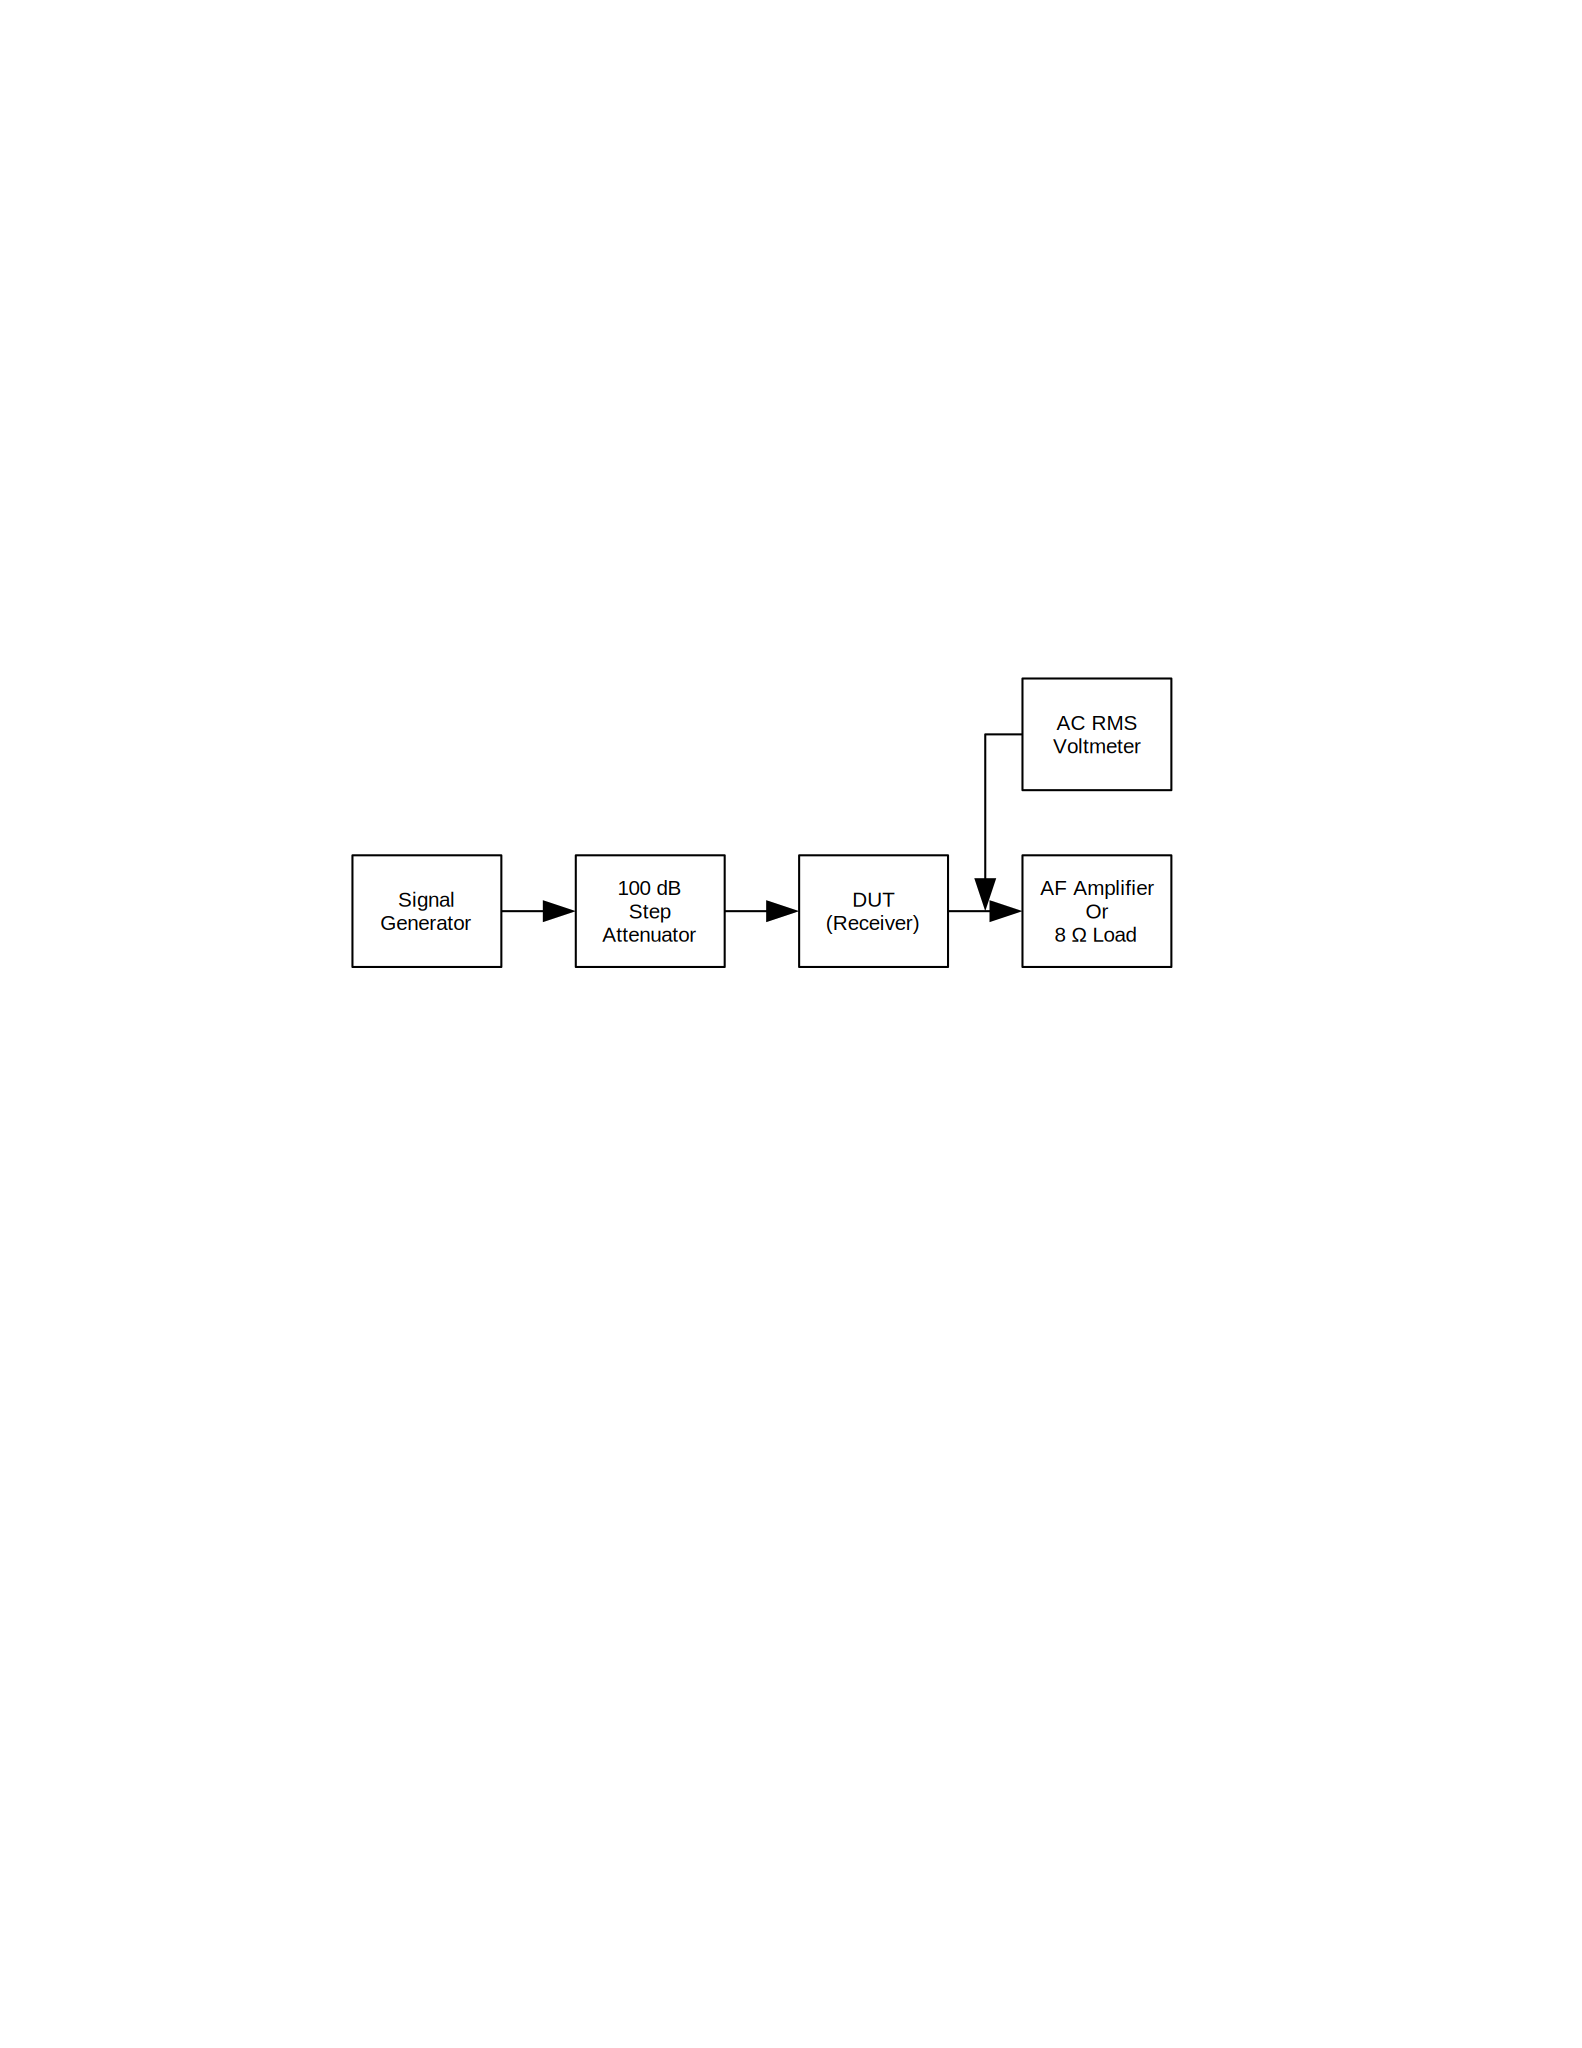
\includegraphics[scale=1]{Illustrations/MDSSetup}
\caption{MDS Measurement Setup}
\end{figure}
\subsubsection*{Required Cabling}
\begin{itemize}
	\item 2 --- 50 $\Omega$ jumper cables \\
		Usually coaxial cables (such as RG-58) with BNC Male-to-BNC Male connectors
	\item 1 --- audio jumper cable \\
		Varies depending on the connectors on your receiver and AF amplifier or load
	\item 1 --- set of voltage probe test leads \\
		Your choice of connector for measuring AC RMS voltage output
\end{itemize}
\subsubsection*{Connections}
\emph{Make sure all equipment is powered off before making any connections.}
\begin{itemize}
	\item Connect the signal generator output to one port of the step attenuator using a 50 $\Omega$ jumper cable.
	\item Connect the other port of the step attenuator to the DUT (receiver) using a 50 $\Omega$ jumper cable.
	\item Connect the audio output of the DUT (receiver) to the AF amplifier or 8 $\Omega$ load using an audio jumper cable.
	\item Connect the AC RMS voltmeter probes to the properly loaded audio output of the DUT (receiver).
\end{itemize}
\subsubsection*{Presets}
\begin{itemize}
	\item Turn ON the signal generator but make sure that the output is OFF. Set the output level to -50 dBm (if you are able to). Set the output frequency to the desired test frequency.
	\item Set the step attenuator for -40 dB. This will give an initial test signal level of -90 dBm. If you are not able to set your signal generator to -50 dBm, set the step attenuator to give you -90 dBm of test signal output.
	\item Turn ON the AF amplifier.
	\item Turn ON the DUT (receiver) and set for the desired measurement band and frequency. Set the AF gain (volume) control fully-counterclockwise (no AF output), then set to an appropriate level for normal listening. If your receiver has AGC, disable it.
	\item Turn ON the AC RMS voltmeter. Set the meter scale as necessary.
\end{itemize}
\subsection*{Test Procedure}
\begin{enumerate}
	\item Turn ON the signal generator output. You should hear a CW tone from the AF amplifier.
	\item Fine-tune the tune control of the DUT (receiver) until the CW tone is centered in the passband and is at maximum level.
	\item Turn OFF the signal generator output.
	\item Note the reading of the AC RMS voltmeter in dB. If the meter reading is fluctuating quite a bit, you may need to increase the AF gain control of the DUT (receiver) in order to get a more stable reading. \\ \\ \\
	AF Noise Power $\rule{3cm}{0.1mm}$
	\item The MDS level will be the AF power level 3 dB higher than the measurement made in the previous step. Calculate it below. \\ \\ \\
	AF Noise + MDS Signal Power $\rule{3cm}{0.1mm}$
	\item Turn ON the signal generator output. The reading from the AC RMS voltmeter should be significantly higher than the calculated level in step 5 (if you are using an external AF amplifier, you may need to turn down its gain control). Use the controls on the step attenuator to step down the test signal level until you have a reading on the AC RMS voltmeter that is closest to the figure derived in previous step. Note the amount of attenuation set on the step attenuator, then subtract that from the output level of the signal generator. This is your MDS figure. \\ \\ \\
	MDS $\rule{3cm}{0.1mm}$
\end{enumerate}
\emph{For example, if your signal generator is set to -50 dBm and the step attenuator is set to 81 dB, then your MDS is -131 dBm.}
\subsection*{Hints and Tips}
\begin{itemize}
	\item Many QRP receivers and transceivers have a relatively low-level audio output, designed for either headphones-only or for a small speaker. In order to make the most accurate measurement, you may need to turn the AF gain control to maximum.
\end{itemize}





\section{IF Rejection}

\subsection*{Overview}
The purpose of this test is to measure the level a CW signal on the IF frequency can bleed into an receiver and get detected as a valid signal. This is defined as a signal on the IF frequency at the receiver antenna port which produces the same amount of AF power output as the intrinsic background noise of the receiver.  For this procedure to work its important to have preformed the MDS measurement as outlined earlier in this document or the noise figure measurement. 
\subsection*{Equipment List}
\begin{itemize}
	\item RF Signal Generator
	\item 100 dB Step Attenuator (at least 1 dB steps required)
	\item AC RMS Voltmeter%(preferably with dB scale)
	\item AF Monitor Amplifier or 8 $\Omega$ Resistive Load
\end{itemize}
\subsection*{Test Setup}
\begin{figure}
\centering
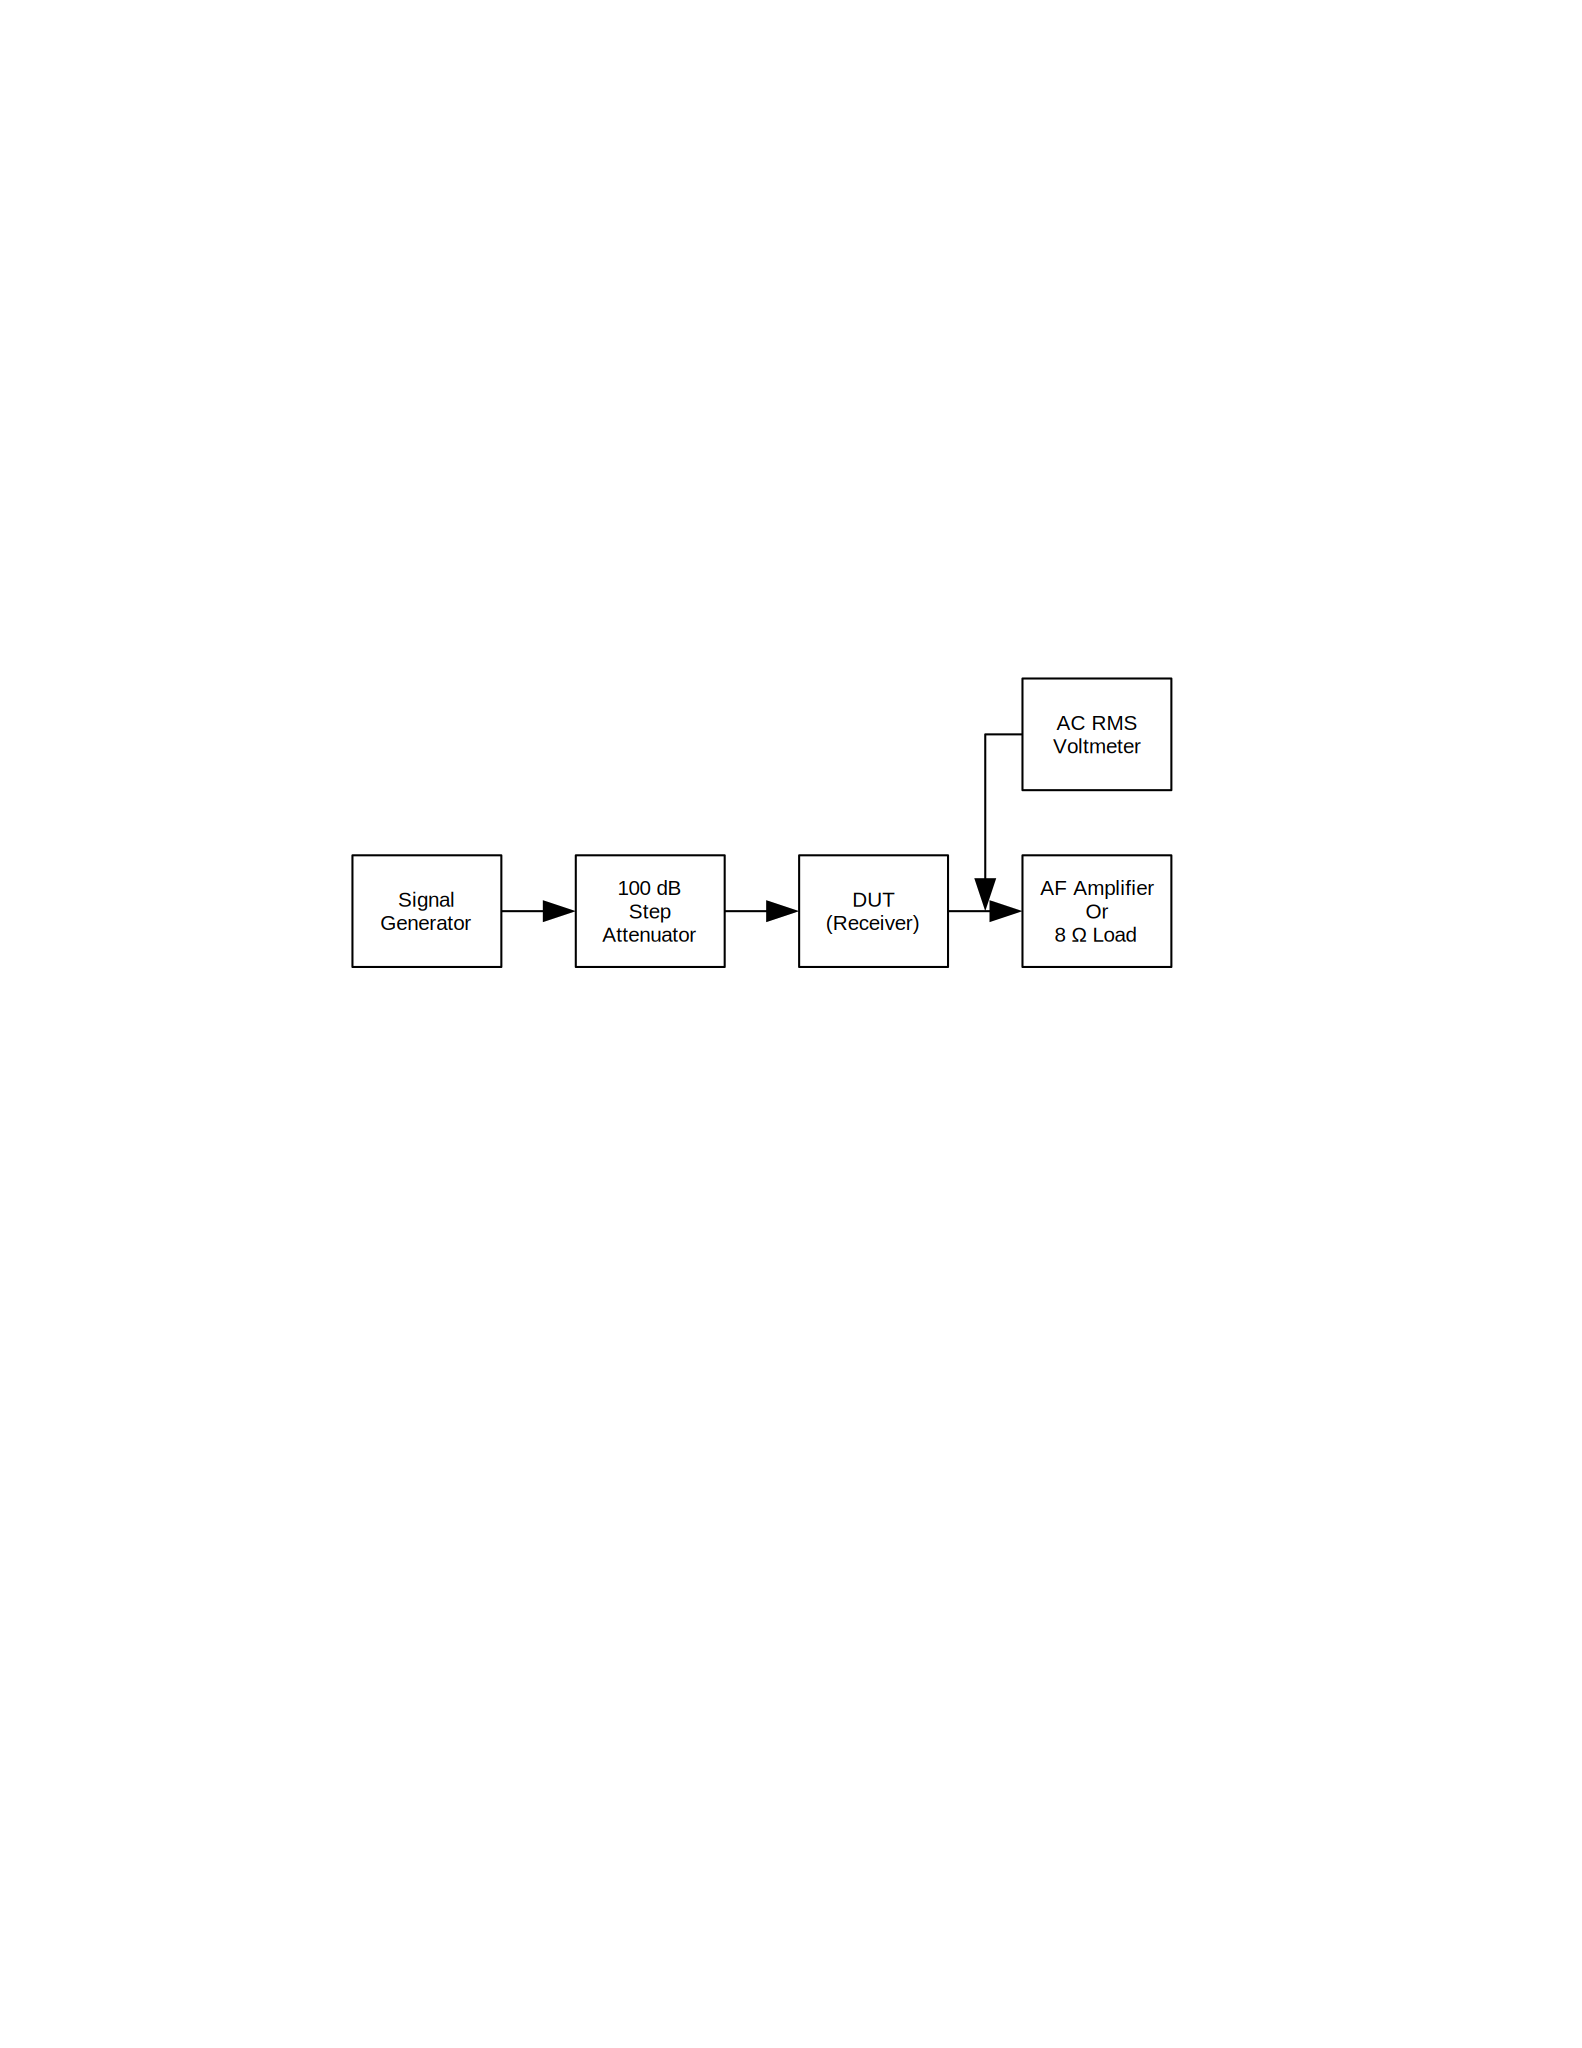
\includegraphics[scale=1]{Illustrations/MDSSetup}
\caption{IF Rejection Setup}
\end{figure}
\subsubsection*{Required Cabling}
\begin{itemize}
	\item 2 --- 50 $\Omega$ jumper cables \\
		Usually BNC Male-to-BNC Male
	\item 1 --- audio jumper cable \\
		Varies depending on the connectors on your receiver and AF amplifier or load
	\item 1 --- set of voltage probe test leads \\
		Your choice of connector for measuring AC RMS voltage output
\end{itemize}
\subsubsection*{Connections}
\emph{Make sure all equipment is powered off before making any connections.}
\begin{itemize}
	\item Connect the signal generator output to one port of the step attenuator using a 50 $\Omega$ jumper cable.
	\item Connect the other port of the step attenuator to the DUT (receiver) using a 50 $\Omega$ jumper cable.
	\item Connect the audio output of the DUT (receiver) to the AF amplifier or 8 $\Omega$ load using an audio jumper cable.
	\item Connect the AC RMS voltmeter probes to the properly loaded audio output of the DUT (receiver).
\end{itemize}
\subsubsection*{Presets}
\begin{itemize}
	\item Turn ON the signal generator but make sure that the output is OFF. Set the output level to -30 dBm (if you are able to). Set the output frequency to the desired test frequency.
	\item Set the step attenuator for -40 dB. This will give an initial test signal level of -70 dBm. If you are not able to set your signal generator to -50 dBm, set the step attenuator to give you -70 dBm of test signal output.
	\item Turn ON the AF amplifier.
	\item Turn ON the DUT (receiver) and set for the desired measurement band and frequency. Set the AF gain (volume) control fully-counterclockwise (no AF output), then set to an appropriate level for normal listening. If your receiver has AGC, disable it.
	\item Turn ON the AC RMS voltmeter. Set the meter scale as necessary.
\end{itemize}

\subsection*{Test Procedure}
\begin{enumerate}
	\item Turn ON the signal generator output and reduce the attenuation. You should hear a CW tone from the AF amplifier. Adjust the frequency so the tone is sentered in the receiver's passband. \\ \\ \\
	IF center frequency $\rule{3cm}{0.1mm}$ MHz.

	\item Turn OFF the signal generator output.

	\item Note the reading of the AC RMS voltmeter in dB. If the meter reading is fluctuating quite a bit, you may need to increase the AF gain control of the DUT (receiver) in order to get a more stable reading. \\ \\ \\
	AF noise power $\rule{3cm}{0.1mm}$ 

	\item 4. The IF rejection power level will be the AF power level 3 dB higher than the measurement made in step 4. Calculate it below.\\ \\ \\

AF Noise + IF rejection power level $\rule{3cm}{0.1mm}$ 

	\item Turn ON the signal generator output. The reading from the AC RMS voltmeter should be significantly higher than the calculated level in step 4 . Use the controls on the step attenuator to step down the test signal level until you have a reading on the AC RMS voltmeter that is closest to the figure derived in step 4. Note the amount of attenuation set on the step attenuator, then subtract that from the output level of the signal generator. This is your IF rejection power level in dBm.\\ \\ \\
	 IF rejection power: $\rule{3cm}{0.1mm}$ dBm.
	 
	\item 6. The total IF rejection is now calculated by subtracting the IF rejection power level from the MDS of the receiver. \\ \\ \\
	 IF rejection: $\rule{3cm}{0.1mm}$ dB.


	\emph{For example, if your signal generator is set to 0 dBm and the step attenuator is set to 43 dB, then your IF rejection power level is -43dBm. With an receiver MDS of -131dBm the IF rejection will then be: -43dbm -(-131dBm)=88dB.}
\end{enumerate}

\subsection*{Hints and Tips}
\begin{itemize}
	\item Many QRP receivers and transceivers have a relatively low-level audio output, designed for either headphones-only or for a small speaker. In order to make the most accurate measurement, you may need to turn the AF gain control to maximum.
	\item If the noise vary to much for your readings to be stable, a low pass integrating filter will smooth out the noise and give a stable reading. A suitable filter is a resistor of 10 k in series with the signal lead and a 1 $\mu$F capacitor, if the noise vary to much increase the capacitor to 10 $\mu$F.  
	\item The IF rejection is the product of the mixer balance and the filter attenuation. Improving the mixer balance will improve the IF rejection.
\end{itemize}





\section{Image Rejection}
\section{Opposite Sideband Rejection}
\section{Two-Tone Third Order Dynamic Range}
\section{Blocking Gain Compression}
\section{Noise Figure}
%This is quite easy to do, will make the text later
\section{Audio Frequency Response}
\section{Audio Power Output}
\chapter{Transmitter Measurements}
blah
\section{Transmitter Power Output}
\section{Transmitter Spectral Purity}
\section{Transmitter Carrier and Unwanted Sideband Suppression}
\section{Transmitter Two-Tone Intermodulation Distortion (IMD)}
\section{Transmitter CW Keying Waveform}
\chapter{Components and Circuits}

\section{Crystal Parameters}
%lots of choises here
\section{Third-Order Intercept}
\section{Noise Figure}
% this depeends opon what equipment are avaible and what component to be measured, could be its own chapter.
\section{Resonator Q}
% here there are several metthods, we should probably describe them all, as not all are suitable for all components
\chapter{DIY Test Equipment}
blah
\end{document}